\documentclass[12pt, a4paper]{article}
\usepackage[utf8]{inputenc}
\usepackage[T1]{fontenc}
\usepackage[slovene]{babel}
\usepackage{times}
\renewcommand{\familydefault}{\rmdefault}
\usepackage{amsmath}
\usepackage{eurosym}
\usepackage{hyperref}
\usepackage{graphicx}
\usepackage[top=2.5cm, bottom=2.5cm, left=3cm, right=2.5cm]{geometry}
\usepackage{indentfirst}
\setlength{\parindent}{0.5cm}


\newcommand{\novukaz}[2]{\underline {#1} \textit{#2}}

\newcounter{stevec}

\newenvironment{novookolje}[2]{\stepcounter{stevec} #1 #2 \thestevec}{}

\begin{document}

\begin{titlepage}
\begin{center}

\large
Univerza v Ljubljani\\
\normalsize
Fakulteta za matematiko in fiziko\\

\vspace{3 cm} 

\large
Eva Deželak in Ines Šilc\\

\vspace{0.5cm}
\LARGE
\textbf{Univerzitetne fundacije}

\vspace{0.5 cm}
\normalsize


\vspace{1.5cm}
\normalsize
SEMINARSKA NALOGA PRI PREDMETU FINANČNI TRGI IN INSTITUCIJE

\vspace{3cm}


\vfill

\large Ljubljana, 2020

\end{center}
\end{titlepage}

\newpage

\tableofcontents

\listoffigures

\newpage

\section{Uvod}

V seminarski nalogi bova raziskali kaj so univerzitetne fundacije, kje se pojavljajo, kakšno je njihovo obnašanje na finančnih trgih, kako so sestavljene njihove naložbene politike in kakšna je dejanska velikost fundacij predvsem v Združenih državah Amerike, kjer so take oblike skladov najizrazitejše ter na koncu še, kako ta sredstva uporabljajo. Raziskali bova podrobno za največji univerzi v Združenih državah Amerike in v Združenem kraljestvu Velike Britanije, kako porabljajo sredstva in kako jih pridobivajo.\\

Najstarejše fundacije, ki so aktivne še danes, so ustanovili kralj Henry VIII in njegovi sorodniki. Njegova babica, grofica Richmond, je ustanovila t.i. \textit{endowed chairs in divinity} na Oxfordu in Cambridgu, Henry VIII pa je na obeh ustanovil t.i. \textit{professorships in a variety of disciplines}. Prvo zabeleženo fundacijo pa je ustanovil Marcus Aurelius za višjo šolo filozofije v Atenah leta 176. \cite{Investopedia}

\section{Kaj so univerzitetne fundacije, njihov namen in delovanje}


Fundacije predstavljajo denar ali druga finančna sredstva, ki se donirajo univerzam. Namenjena so investiranju v rast osnovnega kapitala in zagotavljajo dodatni prihodek za prihodnje investicije in izdatke. Običajno fundacijski skladi pri dodeljevanju sredstev sledijo striktnim pravilom z namenom, da ne bi prevzeli preveč tveganja. \\

Fundacija je denarna ali premoženjska podpora neprofitni organizaciji, ki porabi dobiček od naložb za določen namen. Večina fundacij je zasnovana tako, da glavni znesek ohrani nedotaknjen, medtem ko donos od naložbe porabi za dobrodelne namene. \\

Glavni cilj delovanja univerzitetne fundacije je doseči dva cilja: financirati proračun univerze s stabilnimi in naprej določenimi distribucijami ter vzdrževati dolgoročno vrednost fundacije za prihodnje generacije. \cite{harvard-porocilo}

\subsection{Delovanje fundacij}

Večina fundacij ima določene smernice, ki narekujejo, koliko vsakoletnih prihodkov iz naložb lahko porabijo. Na številnih univerzah ta znesek znaša približno 5 \% celotne vrednosti premoženja. Nekatere bolj popularne šole, na primer Harvard, imajo fundacije v vrednosti več bilijonov USD, zato v njihovem primeru 5 \% celotne vrednosti fundacije predstavlja ogromne količine denarja. \cite{Investopedia}\\

Donatorji lahko omejijo način, kako šole porabijo denar z izjavo o naložbeni politiki (ISP). Na primer, donatorji se lahko odločijo, da bodo uporabili del prihodka iz fundacije za štipendije. Razen takih omejitev lahko univerze preostali del dodeljenega zneska uporabijo kot standardni dohodek. Odločitev o tem, ali ga je potrebno porabiti za najem profesorjev, nadgradnjo oziroma popravilo prostorov ali pa financiranje štipendij, sprejmejo učitelji. \\

Dohodki od naložb fundacije lahko tudi znatno znižajo stroške šolnine za študente. Če na primer finančna sredstva univerze prinesejo skupno 150 milijonov USD in imajo 5 \% omejitev porabe, bi to zagotovilo 7,5 milijona USD razpoložljivega dohodka. Če bi univerza prvotno načrtovala 5,5 milijona USD namenjenih sredstev, bi to pomenilo, da bi lahko presežna 2 milijona USD porabila za plačilo drugih dolgov ali stroškov in prihranke lahko prenesla na študente. \cite{Investopedia}\\

Ker pa so univerze odvisne od donosnosti naložb za dodatni dohodek, lahko pride do težav, če naložbe ne prinesejo ustrezne donosnosti. Zato večino fundacij vodijo strokovnjaki.\\


\subsection{Vrste fundacij}
Obstajajo različne vrste fundacij:
\begin{enumerate}
\item \textbf{Terminske fundacije}: te običajno določajo, da se lahko glavnica porabi šele po preteku določenega obdobja ali po določenem dogodku.
\item \textbf{Neomejene fundacije}: to so sredstva, ki jih je mogoče potrošiti, shraniti, naložiti in razdeliti po presoji institucije, ki je prejela donacijo.
\item \textit{Quasi-endowment} ali \textbf{navidezna fundacija}: je donacija iz strani posameznika ali institucije, ki je dana z namenom, da ta sklad služi točno določenemu namenu. Glavnica se običajno obdrži, medtem ko se dobiček porabi ali razdeli po specifikacijah donatorja. Te fundacije so največkrat ustanovljene iz strani institucije, ki bo od njih imela korist preko notranjih transakcij ali z uporabo neomejenih sredstev, ki so že bili dodeljeni tej instituciji.
\item \textbf{Omejene fundacije}: njihove glavnice so zadržane za vedno, medtem ko se dobiček od vloženih sredstev porabi po navodilih donatorja.
\end{enumerate}

Razen v kakšnih posebnih okoliščinah, pogojev ni mogoče kršiti. Če je institucija blizu bankrota ali pa ga je že razglasila, vendar ima še vedno premoženje v fundacijah, lahko sodišče izda doktrino o \textit{cy-prè}-jih \footnote{Izhaja iz francoske besede \textit{aussi près}, kar v slovenščini pomeni \textit{kolikor blizu je lahko}.}, tako da lahko institucija uporabi ta sredstva za boljši finančni položaj, pri tem pa še naprej spoštuje želje donatorja.

\subsection{Razporejenost fundacij po zveznih državah ZDA}

Na sliki \ref{Slika 1}  so prikazane zvezne države ZDA glede na NACUBO\footnote{The National Association of College and University Business Officers} \cite{wiki}, pri čemer svetla barva pomeni, da je v tisti državi majhna vsota vrednosti fundacij, medtem ko temnejša barva predstavlja višjo vsoto vrednosti fundacij za zasebne univerze. Pri tem moramo vedeti, da so zneski, o katerih govorimo pri fundacijah univerz v ZDA, mišljeni v bilijonih USD. Zelo očitno izstopa zvezna država Kalifornija, ki je obarvana najtemnejše, zato lahko predvidevamo, da se tam skupna vrednost fundacij giblje med 34 in 41 bilijonov USD - konkretneje dosegajo kar 40.829 bilijona USD. Takoj za Kalifornijo je druga po vrsti zvezna država New York z 29.668 bilijona USD. Nato sledi zvezna država Delaware, Pensilvanija in Illinois. \\

\begin{figure}[!h]
\centering

\includegraphics[width = 15 cm]{grafi_zemljevidi/zemljevid_zasebnih.png}
\caption{Fundacije zasebnih univerz v letu 2018, vir: Wikipedia}
\label{Slika 1}
\end{figure}


\begin{figure}[!h]
\centering

\includegraphics[width = 15 cm]{grafi_zemljevidi/zemljevid_javnih.png}
\caption{Fundacije javnih univerz v letu 2018, vir: Wikipedia}
\label{Slika 2}
\end{figure}

Na sliki \ref{Slika 2} pa so prikazane skupne vrednosti fundacij javnih univerz po zveznih državah ZDA glede na NACUBO \cite{wiki}. Kot vidimo, zelo jasno izstopa zvezna država Teksas, kjer prejmejo skupno kar 45.790 bilijonov USD fundacij, precej za Teksasom pa je Kalifornija z 17.666 bilijonov USD fundacij. Nato sledijo še Pensilvanija, Virginija in Michigan. \\

Na podlagi tega lahko sklepamo, da je v Teksasu največ javnega šolstva, hkrati pa vidimo, da je tudi na zemljevidu fundacij zasebnih šol Teksas nekje na zlati sredini glede na skupno število fundacij v zvezni državi, zato bi lahko rekli, da je v Teksasu šolstvo zelo močno zastopano. Je pa pri tem seveda potrebno upoštevati, da je to tudi precej velika zvezna država. \\

Prav tako v obeh primerih Kalifornija nastopa zelo visoko, kar ponovno poudari dejstvo, da je tam šolstvo zelo pomembno in veliko vlagajo vanj. Če primerjamo oba zemljevida med seboj, opazimo še, da je večina fundacij skoncentriranih na vzhodu ZDA (z izjemo Kalifornije, ki kot že rečeno, v obeh primerih stopa precej visoko). Porazdelitev fundacij je skladna tudi s številom prebivalstva v teh predelih Združenih držav.\\

\begin{figure}[!h]
\centering
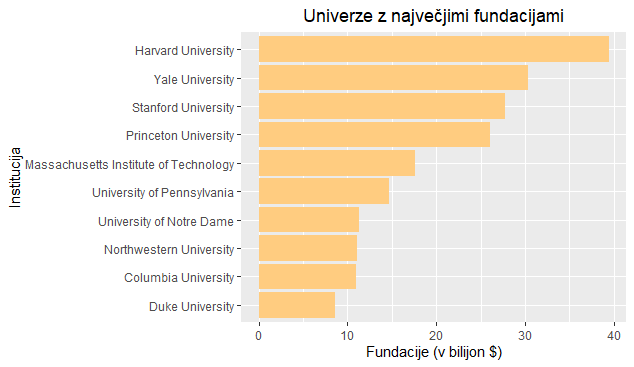
\includegraphics[width = 15 cm]{grafi_zemljevidi/top10.png}
\caption{Najboljših 10 univerz glede na višino fundacij v letu 2018, vir: Wikipedia}
\label{Slika 3}
\end{figure}

Oglejmo si še vrednosti posameznih univerz. Slika \ref{Slika 3} nam prikazuje univerze v ZDA z največjimi fundacijami \cite{wiki}. Kot pričakovano, je tukaj na prvem mestu Harvard, nato sledi Yale, Stanfort in Princeton, ki so tudi najbolj poznane. Pri tem vidimo, da je Harvard daleč v ospredju in dosega skoraj 40 bilijonov \$ fundacij v letu 2018 - natančneje 39.428 bilijonov USD. Ostale tri omenjene univerze pa se gibljejo precej skupaj, in sicer Yale z 30.314
bilijonov USD, Stanford z 27.7 bilijona USD in Princeton z 26.116 bilijona USD.



\section[Naložbene politike univerzitetnih fundacij]{Naložbene politike univerzitetnih fundacij}

Naložbene politike morajo biti zasnovane tako, da zagotavljajo primerno rast in predvidljivost letnih izplačil. Večna narava sklada zagotavlja tako priložnosti kot izzive. Priložnost je v zmožnosti zajemanja z zapletenih, nelikvidnih ali dolgoročnih naložb, za katere je mogoče pričakovati, da bodo prinesle boljše donose. Zgodovinsko je odgovornost skrbnika sklada zahtevala ohranjanje prvotne vrednosti korpusa, kar je običajno povzročilo velike dodelitve obveznicam, denarnim ekvivalentom in drugim naložbam z nizkim tveganjem. Danes si skrbniki skladov svojo minimalno odgovornost razlagajo kot ohranjanje dejanske vrednosti, prilagojene inflaciji, in letni prenos v poslovni proračun. Ta koncept je znan kot generacijska pravičnost ali \textit{generational equity}, ki nakazuje, da je treba prihodnjim generacijam upravičencev do sredstev zagotoviti vsaj enako raven podpore, kot jo uživajo sedanji upravičenci. Stopnja trajnostne porabe sklada mora biti enaka pričakovani skupni donosnosti obdavčenih sredstev, zmanjšani za predvideno stopnjo inflacije. Taka politika zahteva veliko predvidljivost, prvič morajo biti pozorni na napovedovanje inflacije in predvideti morajo skupno donosnost. \\

Ko se dogovorijo glede potrošnje, se morajo dogovoriti glede naložbenih politik. Pogosto se za odločijo, da bodo v naslednjem semestru potrošili 5 \% povprečne vrednosti sklada zadnjih treh fiskalnih let. Nekatere institucije se odločijo samo povečati potrošnjo za toliko, kolikor se je povečala inflacija, kar povzroči predvidljiv tok dohodkov na operativni proračun. \cite{investment1}\\

Fundacije velikokrat niso obdavčene, saj so lahko del institucije, ki ni obdavčena, ali pa so same po sebi neobdavčene. To omogoča višje prihodke, saj ne potrebujejo prenesti deleža dohodkov državi. Primerjave se pogosto izvajajo med zasebnimi fundacijami in univerzitetnimi fundaciji, zlasti pri obravnavi določenih politik (na primer zahteve za izplačilo). Za razliko od zasebnih fundacij se za fundacije fakultet ne zahtevajo izplačila. Zasebne fundacije se razlikujejo od javnih dobrodelnih organizacij, ki so oproščene davkov, in sicer po ozkih osnovah nadzora in finančne podpore.\\

V zgodnjih letih prejšnjega desetletja je prišlo do sprememb, kam se vlagajo sredstva fundacij. Med letoma 2002 in 2010 se je delež naložbenih sredstev, vloženih v lastniške deleže, zmanjšal s 50 \% na 31 \%. Od leta 2010 se je delež premoženjskih sredstev, vloženih v delnice, povečal na 36 \%. Odstotek sredstev, vloženih v stalni dohodek, se je v obdobju 2002 do 2017 zmanjšal s 23 \% na 8 \%. Medtem ko se je delež sredstev, ki se vlagajo v kapital in stalni dohodek, zmanjšal, se je delež sredstev, vloženih v alternativne strategije, povečeval. Empirične raziskave so iskale, zakaj se je dodelitev sredstev univerzitetnih fundacij premaknila v alternativne naložbe. Eden od možnih razlogov je konkurenca. Obstajajo dokazi, da institucije po navadi povečujejo delež vloženih sredstev v naložbene sklade, da "dohitijo" šole, ki so tekmovalci. Druge raziskave ugotavljajo, da je večja verjetnost, da bodo upravljavci fundacijskih naložb vlagali v alternativna sredstva, če imajo institucije višji in manj variabilen dohodek. Te institucije so morda pripravljene prevzeti večje tveganje, povezano z naložbami v alternativne strategije.\cite{investment2}\\

Glavni dohodek fundacij so pa seveda donacije. Fundacije morajo upoštevati tudi pisne smernice donatorjev v zvezi z dodelitvijo dohodkovnih dajatev za trenutno uporabo. Univerzitetne fundacije imajo tudi dostop do strokovnega znanja, ki ga nudijo investicijski odbori, ki posameznim vlagateljem običajno ni na voljo. Univerze se ponašajo z ogromnimi socialnimi omrežji, ki jim omogočajo večji dostop do številnih ključnih naložbenih priložnosti.
Donacije so tudi oproščene državnih davkov, kar jim daje višje donose. Najbolj uspešne fundacije imajo dostop do alternativnih naložb, ki zahtevajo daljša obdobja naložbe in višje minimalne naložbe, kot si jih lahko privošči večina posameznih vlagateljev. \cite{Investopedia2}

\section[Odzivnost na finančne šoke]{Odzivnost na finančne šoke}

Univerzitetne fundacije kažejo na asimetričen odziv na pozitivne in negativne finančne pretrese. Po pozitivnih šokih po navadi sledijo njihovim navedenim politikam izplačil (npr. izplačajo 5 \% preteklega triletnega povprečja vrednosti dobička fundacije). Medtem ko po negativnih šokih številna sredstva aktivno odstopajo od svojih navedenih pravil o izplačilih, dejansko znižujejo stopnjo izplačil na raven, ki je nižja od običajnih pravil ravnanja. Ne najdemo doslednih dokazov, da univerze spreminjajo izplačila darov, da bi nadomestile šoke v druge vire univerzitetnih prihodkov, torej vedenje fundacij ni v skladu s hipotezami glajenja ali samozavarovanja.\\

V literaturi ni soglasnega stališča o tem, kako določiti ciljne funkcije univerz ali fundacij, ki bi jim pomagale pri njihovi podpori. To pomanjkanje soglasja ni posledica pomanjkanja pozornosti, saj je več vodilnih ekonomistov predlagalo normativne modele obnašanja. \\

Prva teorija o fundacijah trdi, da bi morali skrbniki fundacijskih institucije ravnati, kot da je ustanova nesmrtna, in si prizadevati enako obravnavati vse generacije. Tako njegov model predlaga, da bi se skrbniki morali obnašati, kot da imajo ničelno subjektivno časovno prednost. Trenutna potrošnja ne bi smela imeti koristi od prihodnjih daril v fundacije, prav tako ne bi smele vplivati na spremembe šolnin, nepovratnih sredstev ali drugih prihodkov. Ta model ima dve posledici. Prvič, kratkoročni odziv na izplačila na šoke bi moral biti majhen, ker bi morale fundacije s časom širiti dobičke in izgube. V skrajnem primeru, če se univerzitetna fundacija ukvarja s popolnim ravnanjem v neskončnem življenju, bi se morale fundacije odzvati na trajne šoke s prilagajanjem ravni izplačil glede na vrednost trajnosti šoka. Drugič, fundacije bi se morale simetrično odzvati na pozitivne in negativne pretrese; to pomeni, da bi morali biti njihovi odzivi na pozitivne in negativne pretrese enake.\\

Druga teorija univerzitetnih fundacij je, da univerzam omogočajo samozavarovanje, na primer dodelitev sredstev za varovanje pred šokom prihodkov ali uporabo fundacije kot oblike previdnostnih prihrankov, ki jih je mogoče izkoristiti, ko so drugi prihodki nepričakovano nizki. Na nepopolnih trgih pa bi morale univerze prilagoditi sočasne stopnje izplačil kot odziv na šoke fundacije in druge prihodke. Zato je lahko ključna vloga pri izplačilih dajatev izravnavanje učinkov začasnih pretresov. Če so hitre prilagoditve drage, lahko fundacije zagotovijo dragoceno likvidnost ob stalnih šokih in zmanjšajo skupne stroške prilagoditve univerz. \cite{soki}\\


\section[Uporaba sredstev]{Uporaba sredstev}

Pri uporabi sredstev sva se osredotočili na primerjavo dveh univerz, in sicer univerze Harvard in univerze Cambridge, saj splošni podatki za vse univerze niso javno dostopni. Za ti dve univerzi sva se odločili, saj je prva vodila na področju ZDA, druga pa v Združenem kraljestvu Velike Britanije. Primerjali bova, ali se pojavljajo kakšna večja odstopanja, glede na to, na katerem področju se univerza nahaja. 

\subsection{Podroben pregled uporabe sredstev univerze Harvard}

Podrobneje si bomo pogledali, kako deluje fundacija univerze Harvard, saj smo že zgoraj govorili o njej. Fundacija univerze Harvard je stalen vir financiranja, ki vzdržuje učiteljsko in raziskovalno poslanstvo univerze. Sestavljene so iz več kot 13.000 skladov, ki so omogočili programe finančne pomoči, odkritja znanstvenih raziskav in podpore profesorjem na najrazličnejših akademskih področjih. Vsako leto se del sredstev dodeli kot letna distribucija za podporo univerzitetnemu proračunu, pri tem pa se vsak presežek te letne dodelitve obdrži v fundaciji, da  lahko skozi obdobje raste in s tem podpira prihodnje generacije. \cite{harvard} \\

Dodelitev iz strani fundacije Harvarda zagotavlja kritičen vir financiranja univerze. V proračunskem letu, ki se je zaključilo 30.~6.~2019, je bilo dodeljenih 1,9 milijarde USD, kar je prispevalo več kot tretjino celotnih poslovnih prihodkov Harvarda v tem letu. Velika večina sredstev je omejena na posebne programe, oddelke in namene (npr. namenske štipendije, ...) in jih je potrebno porabiti v skladu s pogoji, ki jih je določil donator. \cite{harvard} \\

V proračunskem letu 2019 so razdelitve sredstev predstavljale 35 \% prihodkov univerze. Ta sredstva podpirajo skoraj vse vidike delovanja univerze. Dve največji kategoriji sredstev zajemata plače na univerzi, vključno s profesorstvom in finančno pomočjo za dodiplomske študente, podiplomske študente ter študentsko življenje in dejavnosti, kot je razvidno na sliki 4. Harvard ima tudi sredstva, ki podpirajo akademske programe, knjižnice, umetnostne muzeje in številne druge dejavnosti. Iz naslova fundacij pa mora Harvard financirati tudi skoraj dve tretjini svojih operativnih stroškov, ki so v letu 2019 znašali kar 5,2 milijarde USD. \cite{harvard} 

\subsection{Primerjava univerze Harvard in univerze Cambridge}

Na sliki \ref{Slika 4} je prikazana uporaba sredstev univerze Harvard v letu 2019, na sliki \ref{Slika 5} pa je prikazana uporaba sredstev univerze Cambridge v letu 2019. Obe sliki sta pridobljeni iz njihovih finančnih poročil za to leto, saj podatki v drugačni obliki niso javno dostopni. \\


\begin{figure}[!h]
\centering
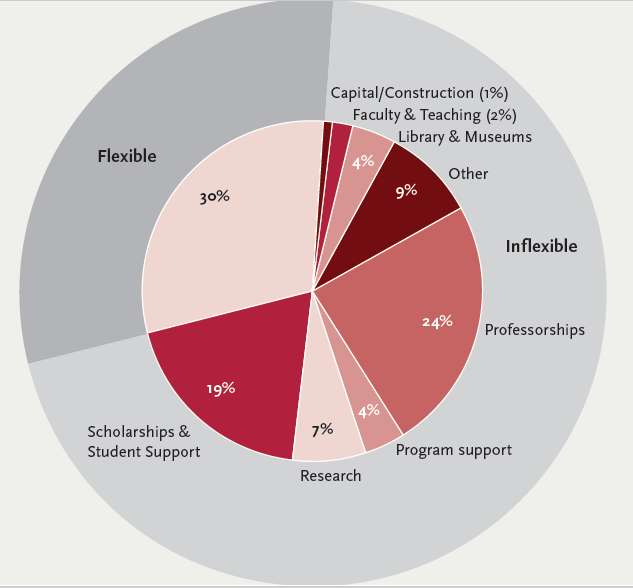
\includegraphics[width = 12 cm]{slike/harvard.png}
\caption{Uporaba sredstev univerze Harvard, vir: Finančno poročilo univerze Harvard}
\label{Slika 4}
\end{figure}


Če kar primerjamo prvi razdelek, torej poučevanje in raziskave, je pri univerzi Cambridge to skupni razdelek in predstavlja 30 \% uporabe sredstev, med tem ko sta ti dve področji pri Harvardu ločeni, skupaj pa predstavljata 9 \%. Tukaj vidimo zelo veliko odstopanje, zato jasno vidimo, da je univerza Cambridge bolj usmerjata v to področje, žal pa iz podatkov ne moremo vedeti, ali več denarja namenja raziskavam ali poučevanju. \\

Naslednji razdelek predstavlja profesorstvo, ki zasede pri univerzi Cambridge 15 \%, medtem ko na Harvardu temu namenijo kar 24 \%. Ponovno vidimo precejšnje odstopanje med univerzama. Kot zadnja primerjava je zanimiv še razdelek štipendij, kjer na univerzi Cambridge namenijo le 5 \% sredstev, ki jih imajo na voljo, medtem ko na Harvardu ta podatek prinese kar 19 \% sredstev. \\

Iz zgoraj primerjanih področji lahko zelo hitro vidimo, da imata obe univerzi precej drugačen pristop. Harvard torej v ospredje postavlja v prvi vrsti profesorje in študente, medtem ko univerza Cambridge največ sredstev nameni raziskovanju in poučevanju ter s tem tudi razvoju naprej. 


\begin{figure}[!h]
\centering
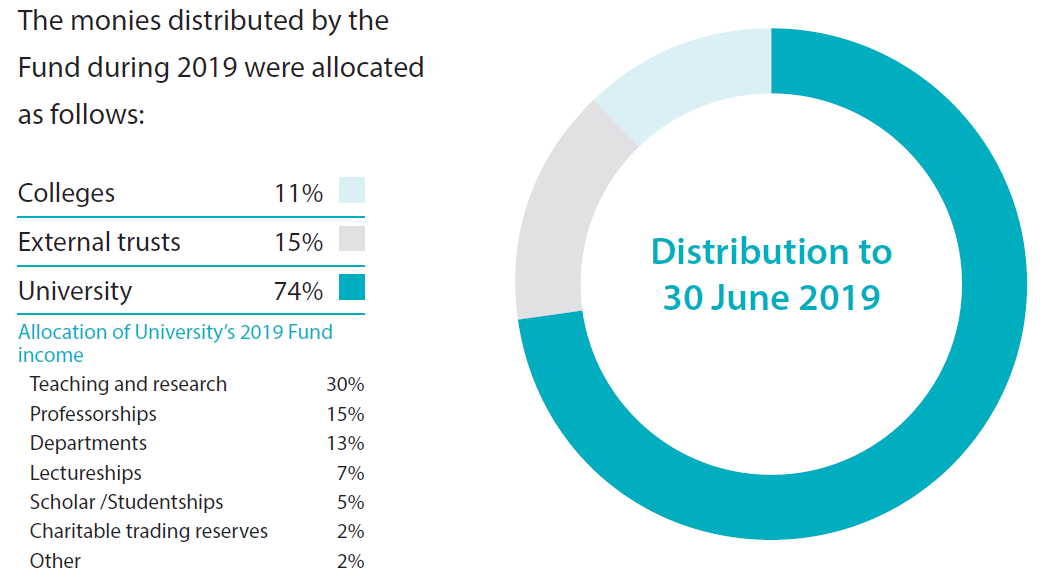
\includegraphics[width = 14 cm]{slike/cambridge.png}
\caption{Uporaba sredstev univerze Cambridge, vir: Finančno poročilo univerze Cambridge}
\label{Slika 5}
\end{figure}


\newpage
\section[Zaključek]{Zaključek}

Uspešna fundacija lahko pomaga zmanjšati finančno breme univerze z ustvarjanjem stalnega pretoka dohodka. Čeprav fundacije na splošno razkrivajo razčlenitve svojih sredstev, vlagatelji morda ne bodo mogli podvajati uspehov, ki so jih že dosegli.\\

Glavni problem in hkrati prednost univerzitetnih fundacij je izredno dolga ročnost oziroma zmožnost naložitve sredstev v investicije z dolgo ročnostjo, saj je zelo malo primerov, ko bi morala univerza dejansko zapreti fundacijo in se znebiti celotnega premoženja. Tako imajo lahko upravljalci fundacij veliko možnosti kam in kako vlagati vsa sredstva. Po navadi gre za velike količine premoženja in so lahko posledično investicijski portfoliji fundacij zelo raznoliki.

\newpage
\section[Viri]{Viri}
\begin{thebibliography}{99}

\bibitem{soki}
Brown, J. R., Dimmock, S. G., Kang, J. K., \& Weisbenner, S. J. (2014). \textit{How university endowments respond to financial market shocks: Evidence and implications}. American Economic Review, 104(3), 931-62.

\bibitem{cambridge-porocilo}
Cambridge Investment Management Limited. (brez datuma). \emph{Cambridge University Endowment Fund, Annual Report 2019}. Pridobljeno 16.~maja~2020 iz \url{https://www.cambridgeinvestmentmanagement.co.uk/files/cuef_annual_report_2019_v2.pdf}.

\bibitem{harvard}
Harvard University. (brez datuma). \emph{Endowment}. Pridobljeno 16.~maja~2020 iz \url{https://www.harvard.edu/about-harvard/harvard-glance/endowment}.

\bibitem{harvard-porocilo}
Harvard University. (2019, 24.~oktober). \emph{Financial report, fiscal year 2019, Harvard University}. Pridobljeno 16.~maja~2020 iz \url{https://www.harvard.edu/sites/default/files/content/fy19_harvard_financial_report.pdf}.

\bibitem{Investopedia}
Investopedia. (2019, 16.~maj). \emph{How do university endowments work?} Pridobljeno 29.~aprila~2020 iz \url{https://www.investopedia.com/ask/answers/how-do-university-endowments-work/}.

\bibitem{Investopedia2}
Investopedia. (2019, 5.~avgust). \emph{How To Invest Like An Endowment?}, Pridobljeno 13.~maja~2020 iz \url{https://www.investopedia.com/articles/financial-theory/09/ivy-league-endowments-money-management.asp}.

\bibitem{investment2}
Sherlock, M. F., Crandall-Hollick, M. L., Gravelle, J., \& Stupak, J. M. (2015). \textit{College and university endowments: Overview and tax policy options. Washington, DC: Congressional Research Service}.

\bibitem{investment1}
Spitz, W. T. (2010). \emph{Investment policies for college and university endowments. Roles and Responsibilities of the Chief Financial Officer: New Directions for Higher Education}, Number 107, 99, 51.

\bibitem{wiki}
Wikipedia: The Free Encyclopedia. (2020, 17.~maj). \emph{List of colleges and universities in the United States by endowment},  Pridobljeno 18.~maja~2020 iz \url{https://en.wikipedia.org/wiki/List_of_colleges_and_universities_in_the_United_States_by_endowment}.

\end{thebibliography}



\end{document}
